\documentclass{mcmthesis}
\mcmsetup{CTeX = false, 
        tcn =57566, problem = B,
        sheet = true, titleinsheet = true, keywordsinsheet = true,
        titlepage = false, abstract = true}
\usepackage{palatino}
\usepackage{array}
\usepackage{indentfirst}
\usepackage{amsmath}
\usepackage{graphicx}
\usepackage{subfigure}
\bibliographystyle{apalike}
\title{An optimized toll plaza design scheme}

\begin{document}

	
	
\begin{abstract}
	
This paper proposes a design scheme for a better shaped and sized toll plaza based on the analysis of vehicle trajectories in an extremely heavy traffic, where the individual vehicles are navigated by a centralized algorithm control. Once the design is generated, a traffic model coded in MATLAB to evaluate and ameliorate the performance of the toll station is simulated.

It is perceived that the boundary of the area where the vehicles actively move is the minimum area required by the normal functionality of toll station. A detailed navigated route is proposed for each vehicle in the area to establish an order among a heavy traffic, which is to successively and non-linearly queue the vehicles into lanes, enabling all those from the tollbooths to successfully merge without causing an accident. 

Using the border of the trajectories as a reference to construct the merging area, calculated on using different time requirements, the shape is then input into the simulation to test for random traffic flows. 

The plaza is simulated by a number of tollbooths of different types, each configurable for vehicle passage type, charging mode and lane direction. The vehicles are simulated by a set of rectangles in a two-dimensional plane, equipped with a moving strategy based on default acceleration and collision avoidance. The vehicles are generated by the tollbooth by a probabilist model, given a fixed traffic flow and then fired for the merge. The vehicles submit to possible collisions with each other  and the road boundary. Both autonomous cars and human-driven cars are simulated, distinguished by adapted moving strategies.

The size of the toll station, run way length and lane numbers are configured by parameters in the simulation, the shape of the station is reflected by the initial speed and direction of the vehicles passing through the specific tollbooth. 

The performance of the design is evaluated by a weighted average of throughput, accident rate statistics and cost. The weights are determined by principal component analysis. Throughput is obtained by calculating the average merging compeletion numbers in reaction to multiple simulated traffic flows. The accident rate is calculated by the collision incidents divided by vehicle quantities. The cost is evaluated by the construction area and tollbooth number. The experiments on $MATLAB$ with different parameters of tollbooth and shape give an analysis of several design schemes, detailed in the report.

In the last part, with different parameters set, an improved design in terms of throughput is proposed on running an optimization algorithm. Various proportions of autonomous vehicles and tollbooths are also tested.

\begin{keywords}
;
\end{keywords}
\end{abstract}

\maketitle
\tableofcontents
\clearpage








\section{A letter to the New Jersey Turnpike Authority}


New Jersey Turnpike Authority,

Our team has proposed an optimized toll station design allowing the increase of throughput and the decrease of cost and accident rate. And a new mathematical model is built in order to help evaluate the performances of designs. 

More specifically, the performance model is developed after taking all important elements related to this problem into consideration, like number of lanes and tollbooths, proportions of tollbooths, varieties of vehicles, change of flows, every decision made on directions and accelerations by drivers . 



\section{Introduction}

\subsection{Statement of the problem}

The design of toll plaza is undoubtedly a state of art as it is hard to find a balance among safety, capacity and cost, facing different situations. It also acts as an essential part in the high-way traffic system. Considering a better toll station design is in demand, mathematical methods and simulation models are implemented to optimize the design schemes, striving to increase the throughput, decrease the cost and accident rate.



\begin{itemize}

\item 
\end{itemize}







\begin{Theorem} \label{thm:latex}

\end{Theorem}

\begin{Lemma} \label{thm:tex}

\end{Lemma}

\begin{proof}
The proof of theorem.
\end{proof}

\subsection{Assumptions}

\begin{itemize}
	\item Assumptions for the toll station:
	\begin{itemize}
         \item Toll station has a fixed configuration for each simulation: vehicle type and charging process.
         \item Tollbooths allowing large vehicles are also available for smaller vehicles to pass.
       	 \item It takes a contain time for every vehicle to leave the tollbooth, an extra delay is caused by the charging process.
	\end{itemize}

    \item Assumptions for the vehicles.
    \begin{itemize}
    	\item The proportions of different types of vehicles are fixed along the time.
    	\item All vehicles are enabled for all 3 types of charging.
    	\item All vehicles leave the tollbooths with a given speed.
    	\item Each vehicle is regarded as a point located in the center of gravity, but the vehicles still have a volume.
    	\item The accelerations of all the vehicles depend on the others who surround themselves.Time is devided into 1 second, drivers' decisions in every second depend on the surroundings and the status are updated every second.
    	\item The biggest wheel steering angle is $45^{\circ}$, and the turning radius is negleted.
    	
    \end{itemize}
    \item Assumptions for the flow generating:
    \begin{itemize}
    \item A fixed total flow $F_t$ is uniformly distributed into seconds, which passes the tollbooths, and then gain the merging flow.
   	\item In cicumstances where traffic is light, the tollbooths the vehicles arrive are random.
    \item In circumsatances where traffic is busy, the vehicles begin to queue up before the tollbooths, therefore every tollbooth is allowing a maximun flow to pass following the proportiional.
    \item Light and heavy traffic is distinguished by a critical flow  $F_c$, which is determined by tollbooth simulation.
    \end{itemize}
	
	
\end{itemize}



Here we list the elements that will influence the throughput of our toll station:
\begin{table}[h]
\centering
   \begin{tabular}{|m{7cm}<{\centering}|p{7cm}<{\centering}|}
   	
   	\hline
   	Notations & Meanings \\
   	\hline
   	$L$ &  Number of lanes \\
   	\hline
   	$B$ &  Number of tollbooths\\
   	\hline
   	$F_t$ & 	 Total flow\\
   	\hline
   	$F_c$ & Critical flow (the maximum of the total flow)\\
   	\hline
   	$P_l$,  $P_m$, $P_s$ & Probability of large-scale automobiles, midium-sized vehicles and compact cars\\
   	\hline
   	$v_{this}$, $a_{this}$ & Speed and acceleration of the vehicle we study\\
   	\hline
   	$v_n$, $a_n$ &  Speed and acceleration of the other vehicles which surround the vehicle we study\\
   	\hline
   	$pos_x$, $pos_y$ & We build a rectangular coordinate system  with the leftmost tollbooth constructed as the origin.\\
   	\hline
   	$L_{length}$ & Merging area length \\
   	\hline
   	$W_{lane}$ & lane width \\
   	\hline
   	
   \end{tabular}
\end{table}\\





\section{Analysis of the Problem}
To respect the notion of "barrier", and to avoid the complexity of gradient, this article discusses only the toll stations of one storey. It is considered that the approach ramps would complicate the traffic flow in both edge of the station, and the cost would be enormous.

\begin{figure}[htbp]
	\small
	\centering
	\caption{Toll station \cite{note}} \label{fig:Ts}
	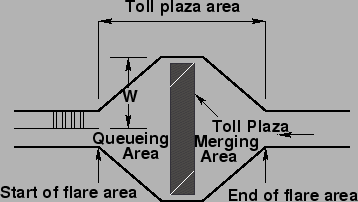
\includegraphics{img3.png}
\end{figure}

In the merging area, all the vehicles merging from $B$ tollbooths into $L$ lanes in a short distance of $L_length$ meters.
With lane width predifined as 2 meters, the merging area is defined as the area surrounded by two curves on a finite two-dimension plane. The curves are represented by two functions, which would be a parameter to be optimized in the problem.

\subsection{Obtaining an adopted shape design}

A primitive idea of establishing an orderly traffic flow is to set up constraints and guidelines for the individualist vehicles: if all participants follow a predefined, well-designed route, there wouldn't be unpredicted crosses at all. It is in addition more practical, to set up such rules in a limited area, where the traffic is limited by the entrance ports of the turnpike.

Thus a design scheme that is capable of coping with the worst traffic conditions, can be inspired by the dynamics of the worst traffic conditions: concurrent vehicles issued from every booth and a high frequency of passages. On finding routing solutions for those vehicle obeying to a centralized control, the convex area covered by the trajectories is the minimum area required by such a traffic in order to merge.

The possible solutions therefore, should guide the vehicles into a proper slot in a queue for each lane, and each vehicle ahead should not be chased by each other, nor the vehicles newly passed through the tollbooth.

Symmetry analyses give that the optimal shape is symmetrical about the central axis of the turnpike. The article concerns therefore only symmetrical.
\begin{figure}
	\begin{minipage}[t]{0.5\linewidth}
		\centering
		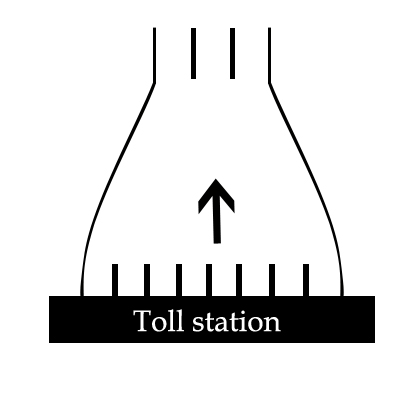
\includegraphics[width=2.2in]{symmetrical.jpg}
		\caption{symmetrical}
		\label{symmetrical}
	\end{minipage}%
	\begin{minipage}[t]{0.5\linewidth}
		\centering
		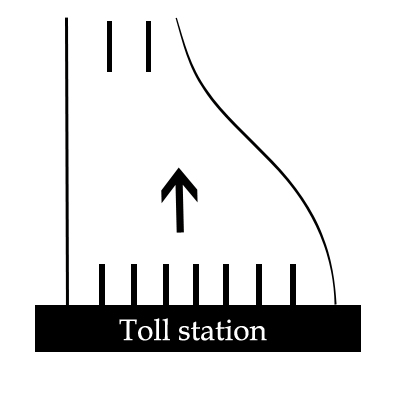
\includegraphics[width=2.2in]{asymmetrical.jpg}
		\caption{asymmetrical}
		\label{asymmetrical}
	\end{minipage}
\end{figure}


\begin{Theorem} \label{thm:yingsongsheng}
The optimal shape is symmetrical about the central axis.
\end{Theorem}

\begin{proof}
Reductio ad absurdum: if the shape is not symmetrical, hence the traffic flow is not symmetrical, so there exist multiple vehicles that have no corresponding vehicles about the axis of symmetry of $L$ lanes. If these vehicles are given slots of certain priority in the queue, and all vehicles successfully merged into $L$ lanes, then the slots of the same priority can also be allocated to the non-existing vehicles in the symmetry. Thus this flow is capable of hold more vehicles, this is not the optimal shape.
\end{proof}

We can furthur show that the comportment of vehicles is also symmetrical about the axis. So only one side of the traffic is to be analysed in the following section.

\begin{Theorem} \label{thm:yingsongsheng2}
The quickest way to merge 2 side-by-side vehicles into 1 lane is to let the vehicles in the lane to be merged to run the most quickily the possible.
\end{Theorem}

[fig C]

\begin{proof}
Denote the direction where the road leads the vertical direction.
Initially, the two vehicles are running side-by-side, and share the same speed $v_0$ and direction.
The vertical distance between the two vehicles (calculated by the position of the center of the vehicle) is 0, the horizontal distance is: $$x_2(t_0)-x_1(t_0)=lane-width$$\\
In the end, vehicle 2 is positioned right after vehicle 1.
$y_1(t_e)-y_2(t_e)=L_d+vehicle_length$\\
The integration of accelerations give the speed at a specific instant:
 $$v_y(t)=v_y(t_0)+ \int_{t_0}^{t}a_y(u)du$$
And the integration of speed give the displacement of a vehicle:
$$y(t)=y(t_0)+ \int_{t_0}^{t}v_y(u)du=y(t_0)+v_y(t_0) \times (t-t_0)+ \int_{t_0}^{t}\int_{t_0}^{w}a_y(u)dudw$$
Equation B can therefore be transcribed as 
[Equa E].
As the intergration reaches for a constant, $t_e$ can be minimised if the difference of the two accelerations can be maximised, from which conclude $a_{y,1}$ to be the maximum value permitted by the situation.
\end{proof}

moving faster in order to outrun the other one, the other is approaching its side. In phase two, the merging vehicle moves behind the other. The minimum time required by phase 1 meets the condition of the previous theorem, meanwhile the minimum time required by phase two is achieved by accelerating to the side then deaccelerate so that the sideway speed is reduced to 0 on arriving in place.

\begin{Theorem} \label{thm:yingsongsheng3}
The queuing strategy can be simplified into a successive merging problem for two vehicles initially run side by side. 
\end{Theorem}

\begin{proof}

on Evaluating the design

\end{proof}
\subsection{Simulation}
In order to evaluate the performance such as throughput, accident rate, this group implements simulation algorithms, mocking the process of vehicles passing through the tollbooth and try to merge without a centralized control: as heavy traffic of everyday definition is not about vehicles of a large size passing the tollbooth continously! The throughput is evaluated by the number of vehicles that successfully enter into the $L$-lane area, and accident rate is calculated by the simulated accident numbers divided by total vehicle numbers.

To begin with, the traffic flow scale is fixed for each simulation experience. $F_t$ stands for the quantity of cars, of various size, passing through the tollbooths every fifteen minutes. The flows of large-scale automobiles, midium-sized vehicles and compact cars are $F_tP_l$, $F_tP_m$, $F_tP_s$.

Since only the traffic after the toll station is to be considered, details of incoming vehicles such as the queuing and proportion distribution are simplified in the model. As the assumptions stated, the proportion of vehicle size and the capability of autonomous driving are implemented by a probabilist model, of which the proportions are fixed by us. 

The vehicles are instancialized with concrete parameters after the tollbooth. That is to say, the traffic to be simulated in the experiences has only one parameter to be adjusted in the performance evaluation: the flow. Corresponding to each flow level, the simulation algorithm adjusts its strategy to generate the traffic. It is remarked that different vehicles takes different times to leave the booth, and the time difference arised by different charging method is also taken into consideration by adding a minimum time gap for each booth to allow the next passage.

The strategy is detailed as follows: for a fixed number of tollbooths in one performance evaluation experience, the maximum traffic is generated by allowing the passage of a maximum of vehicles through each tollbooth. Thus a critical flow $F_c$ denotes the expectation of maximum traffic. 

On cases where traffic flow configured for the simulation is greater than the critical flow, as assumed the traffic flow successfully finds an optimal queuing strategy, allowing each tollbooth to let pass vehicles continously meanwhile respecting the time gap for each vehicle. 

For other cases, the traffic is allocated into each second of the 15 minutes following a uniform fashion. With the assumption that all the vehicles arriving at the booth finds an approriate booth to pass through, and if the vehicle number in this second depasses the number of the tollbooth available, the extra vehicles are queued into the next second.

The vehicles are tagged with its size and nature whether it is human-driven on leaving the tollbooth. The two kinds of tags are independently proportionally distributed.

The merging flow are constituted by vehicles leaving the tollbooth. Since in the problem we are focusing on individual vehicle comportments in an area of $50m\times200m$, the vehicles are not to be represented by moving points: the direction of the front of the vehicle, the direction of the speed and interactions from all orientations are to be taken into account.

It is suggested that at the moment where the vehicle leaves the booth, its speed and direction are restricted by the booth, since a speed limit is implemented and the car can only follow the shape of the lane passing through the booth. Thus, the shape of the booth are represented by the initial speed and direction of the vehicles. With each design of the toll station, an interpretation of initial speed and direction would be given.

One crucial difference of the model presented compared with the classic ones is that this model preserves the physical dimensions of the vehicle, and enables a relative free movement in a two-dimension plane, instead of a strict restraint of one lane. Another one is that the decisions of all vehicles active on the road are calculated for the same instant in the simulation, instead of updating firstly the followed vehicle then the following vehicle.

The human-driven vehicles are represented in the model by an approximation of their vertical projection, rectangles of different sizes. To implement the dynamics, Nagel-Schreckenberg (NS) model \cite{acelluar}, GM model and CF (car following) model are taken reference to simulate the driving strategies. The model presented by this paper considers the acceleration of each vehicle a compound decision of three factors: avoidance for collision with other vehicles.


In this article, an extented version of Car-following model is proposed, preserving the idea that driving consists of the process of perception, decision making and control. Based on the active vehicles on the road and the road shape, the driver's decision includes acceleration or deacceleration of the direction ahead and the one sideways.
$$[Response]_n= \alpha [Simulus]_n$$
 interpreted as interactions between the vehicles, avoidance for collision with the road boundary, and its intrinsic willingness to achieve a maximum speed. 

The acceleration takes three forms for different cases.

It is considered that on leaving a speed limited zone, the vehicles are supposed to reattain a speed of normal level. This process is simulated by a positive factor of the gap of current speed and the ideal speed. However, the acceleration ahead may cause collision with vehicles in front. For the avoidance, the acceleration decision is made based on avoidance of possible collisions: should the driver preserve its current speed, or do an acceleration, the position of the vehicle in the next moment of decision is to be calculated, and the vehicle would not be in collision with the vehicles in its general front. It is worth noting that if such a vehicle in front doesn't exist, the vehicle would accelerate to a maximum speed.

Thus %(this $\ne$ $n$),
%$$\overrightarrow{a_i(t)}=\overrightarrow{a_{interaction}(t)}=\lambda (v_{this}(t))^m \times \sum_n\frac{v_n(t)-v_{this}(t)}{(d_n(t))^l}\times \overrightarrow{dir_{n,this}(t)}$$
%$$d_{n}(t)=distance_n(t)=\sqrt{\delta pos_x(t)^2+\delta pos_y(t)^2}$$
%$$\overrightarrow{dir_{n,this}(t)}=\frac{(pos_x-pos_{x,n},pos_y-pos_{y,n})}{\parallel (pos_{x,this}-pos_{x,n},pos_{y,this}-pos_{y,n}) \parallel} $$
If $\frac{v_y^2-v_{y-forward}^2}{2a_{max}}<distance_{forward}$,
$$v_{y-forward}= \left\{ 
\begin{aligned}
v_{y-forward} \qquad (car)\\
0 \qquad (boundary)
\end{aligned}
\right.
$$

Then for $a_y$:
$$\frac{(v_y+a_yt)^2-v_{y-forward}^2}{2a_{max}}=distance_{forward}$$
if $a_y>a_{max}$, then $a_y=a{max}$, $a_x=0$.\\

If a collision is predicted for current speed, the driver would take neccessary measures to avoid the collision: firstly try to take another lane, or secondly if there's no other choice, slow down. In our model, taking another lane is generalized into taking a left or right angle.

To make the choice of taking another line possible, there should in the first place exist a lane to be taken. In order to keep the vehicles in the simulation from colliding with the edge of the road, a safe-distance psychological model, that the drivers drive away from the edge of the road, if the distance between the vehicle and the boundary is too small, is implemented. 

Secondly, directing the vehicle to the left-front or right-front causes possible collision with other vehicles. The simulation implements a searching algorithm that the vehicle is to search the possibility to turn left or turn right.Firstly We assume that all the drivers know the speed of other vehicules around, which is correspond to the real case. Secondly, we assume that when turn left or turn right, all the vehicles are to preserve its current speed ahead. Thirdly, we neglect the time of the turning action, the $Pos_x$ can change 4m in the next iteration(1 Second).

thus, $\forall j  (j \neq this) $ if
\begin{itemize}
		\item $Pos_{future of j}$ and $ Pos_{future of i}$ are not collided, judging with a extra margin $\Delta l$ to eliminating the deviation of speeds.
		\item $v_{y,this} < v_{y,j} $
		\item $Pos_{future \_ of \_ j} + v_y^2/{2a_{brake \_ maximum}^2} * \overrightarrow{e_y}$ is not out of boundary
		\\ \\ \emph{The third condition ensures that after the vehicle changing a lane, it can stop with the maximaum braking acceleration before colliding with the boundary. }
\end{itemize}

If the left/right lane satisfies these conditions, then the vehicle will move left/right 4 meters ( the width of a lane).

In addition, we consider that $v_{y,this}$ will not change ($a_{y,this} = 0$), except for the case where $v_{y,this} = 0$(when it is waiting for the opportunity to turn). In this special case, we set $a_{y,this} = 1/2 * a_{max \_ acceleration}$.

Thus, \\
$$Pos_{future\_of\_this\_x} = Pos_{future\_of\_this\_x} \pm 4$$\\
$$\left\{ 
\begin{aligned}
a_{y,this} &= 0 ,   \qquad& (v_{y,this} > 0)\\
a_{y,this} &= \frac{1}{2}\times a_{max \_ acceleration} \qquad &(v_{y,this} = 0)
\end{aligned}
\right.
$$

 $\delta y_{max}=v_yt$, as $a_y=0$ when changing direction.\\


The autonomous vehicles are modelled in a similar way, whereas the extra margin $\Delta l$ are smaller. 

The simulation model is based on a combination of Nagel-Schreckenberg (NS) model \cite{acelluar}, GM model, CF (car following) model, and a strategy called Obstacle Avoidance of a Micro-bus[Fernandez et al.,2013], thus takes many some parameters that is merely experimental.

Thirdly, if the first two strategies can not be applied, the vehicle will brake by the acceleration determinated by $v_{y-{foward}}$ and $distance_{foward}$, waiting for the opportunity to turn left or right.
$$
	a_y = \frac{v_{y-foward}^2 - v_y^2}{2\times(distance_{foward} - distance_{limite})}
$$
	Where $distance_limite$ presents a safe distance.
	The determinated $a_y$ needs to be checked if  $|a_y| > a_{brake_{maximum}} $ 


\begin{figure}[htbp]
	\small 
	\centering
	\caption{Our simulation}
	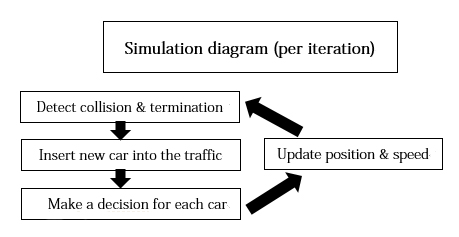
\includegraphics{simulation.jpg}
\end{figure}

\subsection{Evaluating the performance}

In order to propose a better design, the performance of the design can be addressed as a weighted average index of three factors: throughput, accident rate and cost. 

$$Thoughput(flow_total, design) = E_{vehicle number who completes the merge}$$

Accident rate(design) = sum(accidents)/sum(vehicle numbers), sum for all simulation cases

$$Cost(design)=\sum cost_{for booth}(passage type,charge mode,lane length)$$
$$+cost(surface_{whole area} - L_length \times W_lane \times L) $$


\section{Validating the Model}

\subsection{Validating the simulation model}

In order to adjust the parameters and evaluate the performance of the two-dimensional car-following model, motion data of real-life driving must be abundantly supplied to test the model. However, a degradation of dimension can be mocked on setting the tollbooth number $B$ to 1 and the lane number $L$ to 1: the parameters are to be adjusted that the simulated vehicles run similarly with those simulated by a classic car-following model [参考文献,待补充].

After running our program with the numeral coefficient adjusted, the vehicles pulling out of 1 tollbooth to 1 lane will not collide, which indicates our simulation model is correct to some extent.

\subsection{Validating the optimization process}

To optimize the process


\section{The Model Results}




\section{Conclusions}


\section{Strengths and weaknesses}


\subsection{Strengths}
\begin{itemize}
\item \textbf{Applies widely}\\


\end{itemize}
\subsection{Weaknesses}

\begin{appendices}



\end{appendices}


\section{References}
\nocite{*}

\bibliography{math}

	
\end{document}

